\chapter{Provas antigas}

\section{Primeiro semestre, 2011}

{\footnotesize
{\bf C\'alculo I: 1a prova, Turmas D}
\hfill 15 de abril de 2011
\begin{enumerate}
\item (9pts) Dê o domínio da funções $\ln (|2x+1|+3x)\,,\quad \sqrt{\frac{1}{\sen x}}\,,\quad \frac{1}{\ln(1-x^2)}\,.$
\item (10pts) Defina \emph{assíntota horizontal/vertical} de uma função $f$, e 
ache as assíntotas das funções 
$$
%\frac{|x-\pi|}{\pi+x}\,,\quad 
\frac{2+\sen x-3 x^2}{x^2-x+20}
\,,\quad \frac{\sqrt{x(x-1)}}{x-1}\,.$$
\item (6pts) Considere $f(x)=
\begin{cases}
x-\frac{x}{|x|}&\text{ se }x\neq 0\\
-1&\text{ se }x=0\,.
\end{cases}$.
Dê o domínio  $D$ de $f$, assim como o conjunto $C$ dos pontos em que $f$ é contínua.
\item (8pts) Usando a definição de derivabilidade, determine se $f(x)=\sqrt{1-x}$ é derivável nos pontos $a=-1$ e $a=1$, $a=2$.
\end{enumerate}
}

{\footnotesize
{\bf C\'alculo I: 2a prova, Turmas D}
\hfill 27 de maio de 2011
\vspace{2pt}
\begin{enumerate}
\questao{5}{
Um balão esférico se enche de ar a uma taxa de $2$ metros cúbicos por segundo. Calcule
a taxa com a qual o raio do balão cresce no instante em que o seu volume atingiu $\frac{4\pi}{3}$ metros cúbicos.
}{O volume do balão no tempo $t$ é dado por $V(t)=\tfrac43 \pi R(t)^3$. 
Logo, $R(t)=(\frac{3}{4\pi}V(t))^{1/3}$ $\pt{1}$, e pela regra da cadeia, 
$$R'(t)=\tfrac13(\frac{3}{4\pi}V(t))^{-2/3}\frac{3}{4\pi}V'(t)\,.\pt{1}$$
Como no instante $t_*$ que me interessa, $V(t_*)=\frac{4\pi}{3}m^3$, e como $V'(t)=2m^3/s$ para todo $t$, obtemos
$$
R'(t_*)=\tfrac13(\frac{3}{4\pi}\frac{4\pi}{3})^{-2/3}\frac{3}{4\pi}2\,m/s=\frac{1}{2\pi}m/s\pt{3}
$$
Como o Jozelmo mencionou, é claro que o aluno pode também derivar $V(t)=\tfrac43 \pi R(t)^3$ com respeito a $t$ e chegar na resposta. 
Aí, $V'(t)=4\pi R(t)^2R'(t)$ $\pt{2}$, e a juntar tudo pra ter a resposta final dá mais $\pt{3}$. 
}
\questao{8}{Considere um cone de base circular, inscrito numa esfera de raio $R$.
Expresse o volume $V$ do cone em função da sua altura $h$. 
Dê o domínio de $V(h)$ e ache os seus pontos de mínimo e máximo globais. 
Dê as dimensões exatas do cone que tém volume máximo.
}{O volume do cone é dado por $V(h)=\tfrac13 \times \pi r^2\times h$. Mas fazendo um desenho a gente vê que $(h-R)^2+r^2=R^2$. Logo,
$$V(h)=\tfrac{\pi}{3}h(R^2-(h-R)^2)=\tfrac{\pi}{3}(2Rh^2-h^3)\,.\pt{3}$$
O domínio de $V$ é $[0,2R]$ $\pt{1}$.
Os valors na fronteira são $V(0)=0$, $V(2R)=0$.
Procurando os pontos críticos dentro do intervalo: $V'(h)=0$ se e somente se $4Rh-3h^2=0$. Como $h=0$ não está \emph{dentro} do intervalo, somente consideramos o ponto crítico $h_*=\tfrac{4}{3}R$. (Como $V''(h_*)<0$, é máximo local.) Comparando $V(h_*)$ com os valores na fronteira, vemos que $h_*$ é máximo global de $V$ em $[0,2R]$, e que tem dois mínimos globais, em $h=0$ e $h=2R$ $\pt{2}$. \textbf{O maior cone, portanto, tem altura $\tfrac{4}{3}R$ $\pt{1}$, e raio $\sqrt{R^2-(\tfrac{4}{3}R-R)^2}=\frac{\sqrt{8}}{3}R$ $\pt{1}$.}}

\questao{12}{Faça um estudo completo da função $f(x)=\bigl(\frac{x-1}{x}\bigr)^2$, incluindo: assíntotas, variação, posição dos pontos críticos, convexidade, posição dos pontos de inflexão, e grafíco detalhado.}{
O domínio é $D=\bR\setminus \{0\}$, o sinal é sempre não-negativo, tem um zero em $x=1$.
Os limites relevantes são 
$$\lim_{x\to 0^{\pm}}f(x)=+\infty\,,\quad \lim_{x\to \pm\infty}f(x)=1\,.$$
Logo, $x=0$ é assíntota vertical $\pt{1}$ e $y=1$ é assíntota horizontal $\pt{1}$. 
A derivada é igual (em $D$) a $f'(x)=\frac{2(x-1)}{x^3}$ $\pt{1}$ e muda de sinal neste ponto (tabela: $\pt{1}$):
\begin{center}
\begin{tikzpicture}
\tkzTabInit[nocadre,espcl=2,  color, colorV=lightgray!5, colorL=blue!15, colorC=blue!15]
{$x$ /.6,  $f'(x)$ /.9, Variação de $f$ /1.5}%
{,$0$, $1$,}%
%\tkzTabLine{,+,z,+,,+,}
\tkzTabLine{,+,t,-,z,+,}
\tkzTabVar{-/,+/\text{a.v.},-/$0$,+/,}
%\tkzTabLine{,\searrow,\text{mín.},h,\text{mín.},\nearrow,}
\end{tikzpicture}
\end{center}
Coordenadas do ponto de mínimo local: $(1,0)$ $\pt{1}$.
A segunda derivada é dada por $f''(x)=\frac{2(3-2x)}{x^4}$ $\pt{1}$. Ela se anula em $x=\tfrac32$, e muda de sinal neste ponto (tabela: $\pt{1}$):
\begin{center}
\begin{tikzpicture}
\tkzTabInit[nocadre,espcl=2,  color, colorV=lightgray!5, colorL=blue!15, colorC=blue!15]
{$x$ /.6,  $f''(x)$ /.9, Convexidade de $f$ /1.5}%
{,$0$, $\tfrac32$,}%
\tkzTabLine{,+,t,+,z,-,}%
\tkzTabLine{,\text{conv.},t,\text{conv.},z,\text{conc.},}%
\end{tikzpicture}
\end{center}
Coordenadas do ponto de inflexão: $(\tfrac{3}{2},f(\tfrac{3}{2}))=(\tfrac{3}{2},\tfrac19)$ $\pt{1}$.
Agora o gráfico é fácil de montar $\pt{4}$:
\begin{center}
\begin{tikzpicture}[scale=1.3]
%\clip (0.5,0.5) rectangle (1.5,1.5);
%\fill[color=gray!30] (1,0)--plot[domain=1:3](\x,0.6*\x)--(3,0)--cycle;
%\draw [domain=-0.1:3.2] plot (\x,{0.6*\x});
%\draw (1,0) node {$\shortmid$};
\draw [thick, domain=-4:-1.2, samples=100] plot (\x,{(\x-1)^2/\x^2});
\draw [thick, domain=0.4:4, samples=100] plot (\x,{(\x-1)^2/\x^2});
% \draw (0.5,-0.11) node{$\half$};
\draw [>=latex, ->] (-4,0)--(4,0) node[right] {$x$};
\draw [>=latex, ->] (0,-0.1)--(0,3) node[left] {$f(x)$};
\draw [dotted] (-4,1)--(4,1) node[above left] {Assíntota horiz.: $y=1$};
\draw [dotted] (0,0)--(0,3.5) node[right] {Assíntota vertic.: $x=0$};
% \draw [>=latex, ->] (0,0)--(0,1.2); 
% \draw (0,-0.2) node{$0$};
\fill (1,0) circle (0.35mm);
\draw (1,0) node[below] {$(1,0)$};
\fill (1.5,0.1111) circle (0.35mm);
\draw [>=latex, <-] (1.52,0.0911)--(2,-0.3) node[right] {$(\tfrac{3}{2},\tfrac{1}{9})$};
%\draw (1,0) node[below] {mín. $(1,0)$};
% \draw (2,-0.22) node{$1$};
% \draw[dotted] (2,0) arc (0:360:2);
% \draw (2,0) arc (0:90:2);
% \draw (0.8,0.8) node {$A$};
% \draw [>=latex, ->] (0,0)--(0,2.2) ; 
\end{tikzpicture}
\end{center}
}

\questao{8}{Calcule os limites 
$$\lim_{z\to \infty}\bigl(\frac{z+9}{z-9}\bigr)^z\,,\quad\lim_{\alpha\to 0}\frac{1-\cos(\alpha)}{\sen(\alpha+\frac{\pi}{2})}\,,\quad
\lim_{x\to \infty}x^{\ln x}e^{-x}\,,\quad
\lim_{x\to \infty}\frac{\sqrt{2x+1}}{\sqrt{x-1000}}\,.
%\quad\lim_{h\to 0^+}\sqrt{1+h}^{1/h}\,.
$$}{
\textbf{Atenção: sejam exigentes com a lógica! Absurdidades notacionais do tipo 
$$\lim_{x\to 0}\frac{\sen x}{x}=\frac{\cos x}{1}=1$$
têm que ser penalizadas, de alguma forma.}
Detalhei um pouco a pontuação, seguindo as sugestões do Jozelmo e da Larissa. Se faltar um grau de detalhamento, deixo vocês interpolar... 
\begin{align*}
 \lim_{z\to \infty}\bigl(\frac{z+9}{z-9}\bigr)^z&=\exp \Bigl(\lim_{z\to \infty} z \ln \frac{z+9}{z-9}\Bigr)\\
&=\exp \Bigl(\lim_{z\to \infty} \frac{\ln (z+9)-\ln (z-9)}{\frac{1}{z}}\Bigr)\text{ e as hipót. de BH satisfeitas $\pt{0.5}$, logo}\\
&=\exp \Bigl(\lim_{z\to \infty} \frac{\frac{1}{z+9}-\frac{1}{z-9}}{\frac{-1}{z^2}}\Bigr)\pt{0.5}\\
&=\exp \Bigl(\lim_{z\to \infty} \frac{18 z^2}{z^2-81}\Bigr)\\
&=e^{18}\,. \pt{1.5}
\end{align*}
O segundo limite vale 
$$\lim_{\alpha\to 0}\frac{1-\cos(\alpha)}{\sen (\alpha+\pi/2)}=\tfrac01=0\pt{1.5}\,.$$ 
Para o terceiro,
\begin{align*}
 \lim_{x\to \infty}x^{\ln x}e^{-x}&=\exp \Bigl(\lim_{x\to \infty} \big((\ln x)^2-x \big)\Bigr)\\
&=\exp \Bigl(\lim_{x\to \infty} x\big(\frac{(\ln x)^2}{x}-1 \big)\Bigr)\pt{1}
\end{align*}
Usando BH duas vezes, verifica-se que $\lim_{x\to \infty}\frac{(\ln x)^2}{x}=0$ $\pt{1}$, 
logo o limite acima vale $0$ $\pt{0.5}$. Fico feliz se alguém falar que ``qualquer potência do logaritmo cresce mais devagar do que o $x$'', sem outra justificativa desse último passo.\\
O último limite vale (sem usar BH, claro...) 
$$\lim_{x\to \infty}\frac{\sqrt{2x+1}}{\sqrt{x-1000}}=\sqrt{2}\lim_{x\to \infty}\frac{\sqrt{1+\frac{1}{2x}}}{\sqrt{1-\frac{1000}{x}}}=\sqrt{2}\frac{1}{1}=\sqrt{2}\pt{1.5}\,.$$
}
\end{enumerate}
%JUSTIFIQUE TODAS AS SUAS RESPOSTAS!
%\vspace{7mm}
%%%%%%%%%%%%%%%%
%%%%%%%%%%%%%
}

{\footnotesize
{\bf C\'alculo I: 3a prova, Turmas D}
\hfill 1 de julho de 2011
\vspace{2pt}
\begin{enumerate}

\questao{12}{
Calcule as primitivas
$\int e^{2u}\cos(3u)du$ (6pts), $ \int \frac{x^3}{\sqrt{4x^2+1}}dx$ (7pts).}
 {
%Solução: Como $t^4+t^3=t^3(t+1)$, procuramos uma separação da forma 
% $$
% \frac{1}{t^4+t^3}=\frac{A}{t}+\frac{B}{t^2}+\frac{C}{t^3}+\frac{D}{t+1}\,\quad \forall t. \pt{2}
% $$
% Colocando no mesmo denominador e juntando os termos vemos que $A,B,C,D$ têm que satisfazer 
% $$
% 1=(A+D)t^3+(A+B)t^2+(B+C)t+C\quad\forall t\,.
% $$
% Logo, $C=1$, $B=-C=-1$, $A=-B=+1$, e $D=-A=-1$ $\pt{2}$. Isso implica
% \begin{align*}
% \int \frac{1}{t^4+t^3}dt&=\int\frac{dt}{t}-\int \frac{dt}{t^2}+\int \frac{dt}{t^3}-\int \frac{dt}{t+1}\\
% &=\ln|t|+\frac{1}{t}-\frac{1}{2t^2}-\ln|t+1|+C\,.\pt{2}
% \end{align*}
Integrando duas vezes por partes, 
\begin{align*}
 \int e^{2u}\cos (3u)du&=\tfrac12 e^{2u}\cos (3u)-\int \tfrac12 e^{2u}(-3\sen (3u))du\pt{2}\\
&=\tfrac12 e^{2u}\cos (3u)+\tfrac32 \int  e^{2u}\sen (3u)du\\
&=\tfrac12 e^{2u}\cos (3u)+\tfrac32\Big\{\tfrac12 e^{2u}\sen (3u)-\int \tfrac12 e^u(3\cos (3u))du \Big\}\,.\pt{2}
\end{align*}
Rearranjando, 
$$
\int e^{2u}\cos (3u)du=\tfrac{2}{13}e^{2u}\Bigl\{\cos (3u)+\tfrac{3}{2}\sen (3u)\Bigr\}+C\,.\pt{2}
$$
Para a segunda integral, fazendo $x=\tfrac12\tan \theta$ dá
\begin{align*}
 \int \frac{x^3}{\sqrt{4x^2+1}}dx&=\int \frac{(\tfrac12 \tan \theta)^3}{\sqrt{\sec^2\theta}}
\half\sec^2\theta d\theta\\
&=\tfrac{1}{16} \int\tan^3\theta \sec\theta d\theta\pt{3}\\
&=\tfrac{1}{16} \int (\sec^2\theta-1)\sec\theta \tan\theta d\theta
\end{align*}
Com $u=\sec \theta$, essa última integral vale 
$$
\int (u^2-1)du=\frac{u^3}{3}-u+C=
\frac{\sec^3\theta}{3}-{\sec\theta}+C\pt{2}
$$
Mas $\tan \theta=2x$ implica $\sec \theta=\sqrt{1+4x^2}$. Logo,
$$
\int \frac{x^3}{\sqrt{4x^2+1}}dx=\frac{(1+4x^2)^{\frac{3}{2}}}{48}
-\frac{\sqrt{1+4x^2}}{16}+C\,.\pt{2}
$$
Observe que pode também rearranjar um pouco a função e fazer por partes:
\begin{align*}
 \int \frac{x^3}{\sqrt{4x^2+1}}dx&=
 \tfrac14\int x^2\frac{8x}{2\sqrt{4x^2+1}}dx\\
&=\tfrac14\Bigl\{x^2\sqrt{4x^2+1}-\int (2x)\sqrt{4x^2+1}dx\Bigr\}\\
&=\tfrac14\Bigl\{x^2\sqrt{4x^2+1}-\tfrac14\frac{(4x^2+1)^{3/2}}{3/2}\Bigr\}+C
\end{align*}
(Dá na mesma!)
}



\questao{8}{Considere a região $R$ delimitada pelo gráfico da função $y=\sen x$, pelo eixo $x$, e pelas duas retas $x=\pi/2$, $x=\pi$.
Calcule a área de $R$ (4pts). Em seguida,
monte uma integral (não precisa calculá-la) cujo valor dê o volume so sólido obtido girando $R$: 1) em torno do eixo $x$ (2pts), 2) em torno da reta $x=\pi$ (4pts).}{
A área é dada por 
$$\int_{\pi/2}^\pi\sen (x)dx=-\cos (x)|^{\pi}_{\pi/2}=-(-1)-0=1\,.\pt{4}$$
Girando em torno do eixo $x$:
$$
V_1=\int_{\pi/2}^{\pi}\pi(\sen x)^2dx\,.\pt{2}
$$
Ou com as cascas:
$$
V_1=\int_0^12\pi y (\pi/2-\arcsen y)dy\,.
$$
Em torno da reta $x=\pi$, usando as cascas:
$$
V_2=\int_{\pi/2}^\pi2\pi(\pi-x)\sen xdx\pt{4}
$$
Sem usar as cascas:
$$
V_2=\pi(\tfrac{\pi}{2})^2\cdot 1-\int_0^1\pi (\arcsen y)^2dy\,.
$$
}

\questao{8}{Defina o que significa \emph{a integral imprópria $\int_a^\infty f(x)dx$ convergir} (3pts). Em seguida,
determine se as integrais impróprias $\int_1^\infty\frac{dx}{2x^2+1}$ (4pts), 
$\int_3^\infty\frac{\ln x}{x}dx$ (4pts), convergem ou não.
}{
A integral imprópria $\int_a^\infty f(x)dx$ é definida pelo limite
$\lim_{L\to \infty}\int_a^L f(x)dx$. Diz-se que a integral imprópria converge se esse limite existe e é finito $\pt{3}$. 
$$
\int_1^\infty\frac{dx}{2x^2+1}=\lim_{L\to \infty}
\int_1^L\frac{dx}{2x^2+1}=\lim_{L\to \infty}
\int_1^L\frac{dx}{(\sqrt{2}x)^2+1}=\tfrac{1}{\sqrt{2}}\lim_{L\to \infty}\int_{\sqrt{2}}^L\frac{du}{u^2+1}\pt{2}$$
Como o limite
$$\lim_{L\to \infty}\int_{\sqrt{2}}^L\frac{du}{u^2+1}=
\lim_{L\to \infty}\bigl\{\arctan L-\arctan \sqrt{2}\bigr\}=\tfrac{\pi}{2}
-\arctan \sqrt{2}\,$$
existe e é finito $\pt{1}$, a primeira integral converge $\pt{1}$. Observe que podia também comparar $\frac{1}{2x^2+1}\leq \frac{1}{2x^2}$. Como $\frac{1}{x^2}$ é da forma $\frac{1}{x^p}$ com $p>1$, a integral imprópria $\int_1^\infty\frac{dx}{x^2}$ converge, logo $\int_1^\infty\frac{dx}{2x^2+1}$ converge também. (Usar comparação também dá $\pt{4}$; aceito que se use o fato de ``$\int_1^\infty\frac{dx}{x^p}$ convergir'', sem justificativa).
Para a segunda, fazendo $u=\ln x$, 
$$\int_3^\infty\frac{\ln x}{x}dx=\lim_{L\to\infty}\int_3^L\frac{\ln x}{x}dx=
\lim_{L\to\infty}\int_{\ln 3}^{\ln L}udu\pt{2}=\lim_{L\to\infty}\tfrac12\bigl\{
(\ln L)^2-(\ln 3)^2\bigr\}=\infty\pt{1}\,.$$
Logo, $\int_3^\infty\frac{\ln x}{x}dx$ diverge $\pt1$. Podia também comparar $\frac{\ln x}{x}\geq \frac{1}{x}$, e como $\frac{1}{x}$ é da forma $\frac{1}{x^p}$ com $p\leq 1$, a integral imprópria $\int_3^\infty\frac{1}{x}dx$ diverge, $\int_3^\infty\frac{\ln x}{x}dx$ diverge também. ($\pt{4}$, claro)
}


\end{enumerate}
%JUSTIFIQUE TODAS AS SUAS RESPOSTAS!
%\vspace{7mm}

%%%%%%%%%%%%%%%%
}
%%%%%%%%%%%%%



{\footnotesize
{\bf C\'alculo I: Prova suplementar, Turmas D}
\hfill 6 de julho de 2011
\vspace{2pt}
\begin{enumerate}

\questao{6}{Usando a \emph{definição} de derivada, 
calcule a inclinação da reta tangente ao círculo de raio $5$ centrado na origem, no ponto $P=(3,4)$.}{Com $f(x)=\sqrt{25-x^2}$,
\begin{align*}
f'(3)=\lim_{h\to 0}\frac{f(3+h)-f(3)}{h}\pt{1}&=\lim_{h\to 0}\frac{\sqrt{25-(3+h)^2}-\sqrt{25-3^2}}{h}\\
&=\lim_{h\to 0}\frac{\sqrt{16-6h-h^2}-\sqrt{16}}{h}\\
&=\lim_{h\to 0}\frac{(16-6h-h^2-16)}{h(\sqrt{16-6h-h^2}+\sqrt{16})}\\
&=\lim_{h\to 0}\frac{-6-h}{\sqrt{16-6h-h^2}+\sqrt{16}}\\
&=-\tfrac{3}{4}\pt{5}
\end{align*}
Quem fizer $(\sqrt{25-x^2})'|_{x=3}=\frac{-2x}{2\sqrt{25-x^2}}|_{x=3}=-3/4$: ganha $\pt{3}$.
}

\questao{12}{Estude a função $f(x)=\frac{x^2-1}{x^2+1}$: domínio, sinal, assíntotas, tabela de variação, mín./máx. locais, concavidade, pontos de inflexão, gráfico. (ATENÇÃO: verifique duas vezes as contas que envolvem derivadas!)
}{Domínio: $D=\bR$.  Sinal: $f(x)$ é $\geq 0$ se $|x|\geq 1$, $<0$ caso contrário $\pt{2}$. Como 
$$
\lim_{x\to \pm \infty}\frac{x^2-1}{x^2+1}=\lim_{x\to \pm \infty}\frac{1-\tfrac{1}{x^2}}{1+\tfrac{1}{x^2}}=1\,,
$$
a reta $y=1$ é assíntota horizontal, e não tem assíntotas verticais $\pt{2}$.
A derivada se calcula facilmente: $f'(x)=\frac{4x}{(x^2+1)^2}$. Tabela de variação $\pt{2}$:
\begin{center}
\begin{tikzpicture}
\tkzTabInit[nocadre,espcl=2,  color, colorV=lightgray!5, colorL=blue!15, colorC=blue!15]
%{$x$ /.6,  $f'(x)$ /.9, Variação de $f$ /1.5}%
{$x$ /.5,  $f'(x)$ /.5, Var. de $f$ /1}{,$0$,}
%\tkzTabLine{,+,z,+,,+,}
\tkzTabLine{,-,z,+,}
\tkzTabVar{+/,-/\text{min.},+/,}
%\tkzTabLine{,\searrow,\text{mín.},h,\text{mín.},\nearrow,}
\end{tikzpicture}
\end{center}
O mínimo local tem coordenadas $(0,f(0))=(0,-1)$ $\pt{1}$. A segunda derivada é dada por $f''(x)=\frac{4(1-3x^2)}{(x^2+1)^3}$, logo $\pt{2}$:
\begin{center}
\begin{tikzpicture}
\tkzTabInit[nocadre,espcl=2,  color, colorV=lightgray!5, colorL=blue!15, colorC=blue!15]
%{$x$ /.5,  $f''(x)$ /.7, Conc. de $f$ /1.3}
{$x$ /.5,  $f''(x)$ /.5, Conc. de $f$ /1}
{,$-\tfrac{1}{\sqrt{3}}$, $+\tfrac{1}{\sqrt{3}}$,}
\tkzTabLine{,-,z,+,z,-,}
\tkzTabLine{,{\frown},\text{infl.},\smile,\text{infl.},\frown,}
\end{tikzpicture}
\end{center}
Pontos de inflexão: $(\tfrac{-1}{\sqrt{3}},f(\tfrac{-1}{\sqrt{3}}))=(\tfrac{-1}{\sqrt{3}},-\tfrac{1}{2})$, $(\tfrac{+1}{\sqrt{3}},f(\tfrac{+1}{\sqrt{3}}))=(\tfrac{+1}{\sqrt{3}},-\tfrac{1}{2})$ ($\pt{1}$). Gráfico $\pt{2}$:
\begin{center}
\begin{tikzpicture}[scale=1.3]
\draw [thick, domain=-4:4, samples=100] plot (\x,{(\x^2-1)/(\x^2+1)});
\draw [>=latex, ->] (-4,0)--(4,0) node[right] {$x$};
\draw [>=latex, ->] (0,-0.1)--(0,1.5) node[left] {$f(x)$};
\draw [dotted] (-4,1)--(4,1) node[above left] {Assíntota horiz.: $y=1$};
%\fill (1,0) circle (0.35mm);
%\fill (-1,0) circle (0.35mm);
\fill (0,-1) circle (0.35mm);
\draw (0,-1) node[below] {$(0,-1)$};
\fill (-0.577,-0.5) circle (0.35mm);
\draw (-0.577,-0.6) node[left]{$(\tfrac{-1}{\sqrt{3}},-\half)$};
\fill (+0.577,-0.5) circle (0.35mm);
\draw (+0.577,-0.6) node[right]{$(\tfrac{+1}{\sqrt{3}},-\half)$};
\end{tikzpicture}
\end{center}
}

\questao{6}{Calcule a área da região finita delimitada pelo gráfico da função $y=\ln x$ e pelas retas $y=-1$, $y=2$, $x=0$.}{
\begin{center}
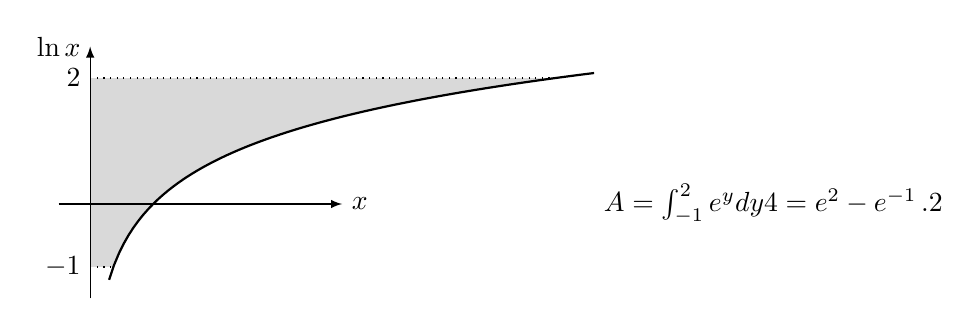
\begin{tikzpicture}[scale=0.8]
\fill[color=gray!30] (0,-1)--(0.368,-1)--plot[domain=0.368:7.38](\x,{ln(\x)})--(0,2)--cycle;
\draw [thick, domain=0.3:8, samples=100] plot (\x,{ln(\x)});
\draw [>=latex, ->] (-0.5,0)--(4,0) node[right] {$x$};
\draw [>=latex, ->] (0,-1.5)--(0,2.5) node[left] {$\ln x$};
\draw [dotted] (0,-1)--(0.368,-1);
\draw [dotted] (0,2)--(7.38,2);
\draw (0,-1) node[left]{$-1$};
\draw (0,2) node[left]{$2$};
\draw (8,0) node[right]{$A=\int_{-1}^2e^ydy\pt{4}=e^2-e^{-1}\,. \pt{2}$};
\end{tikzpicture}
\end{center}
Pode sempre fazer coisas mais complicadas, tipo 
$$
A=\int_0^{e^{-1}}(2-(-1))dx+\int_{e^{-1}}^{e^2}(2-\ln x) dx\pt{4}=(\cdots)=e^2-e^{-1}\pt{2}\,.
$$
}



\questao{8}{Calcule $\int \frac{dx}{x+x^2}$, $\int x e^{-x}dx$.}{A decomposição em frações parciais dá
$$
\int \frac{1}{x^2+x}dx=\int\frac{1}{x(x+1)}dx=\int\Bigl\{\frac{1}{x}-\frac{1}{x+1}\Bigr\}dx\pt{2}=\ln |x|-\ln|x+1|+C\pt{2}\,.
$$
Por partes:
$$
\int xe^{-x}dx=x(-e^{-x})-\int (-e^{-x})dx=-xe^{-x}+\int e^{-x}dx=-xe^{-x}-e^{-x}+C\,.\pt{4}
$$
}
\vspace{1cm}

%aiiiiie

\end{enumerate}

}
